\section{Methodology}
\label{sec:method}

\subsection{Description of the Proposed Project}

\subsubsection{Inputs}

All inputs are public. They are downloaded once in Week 6, and their versions and checksums are recorded so results can be reproduced.

\begin{itemize}
\item \textbf{Human interactome.} The protein--protein interaction graph compiled by Cheng et al.\ \cite{cheng2019combinations}, restricted to its largest connected piece. Using the same graph as \cite{ramos2025quantum} makes our results comparable with theirs. If both projects run, the sister project's BioGRID graph \cite{oughtred2021biogrid} can be used instead.
    \begin{figure}[h]
        \centering
        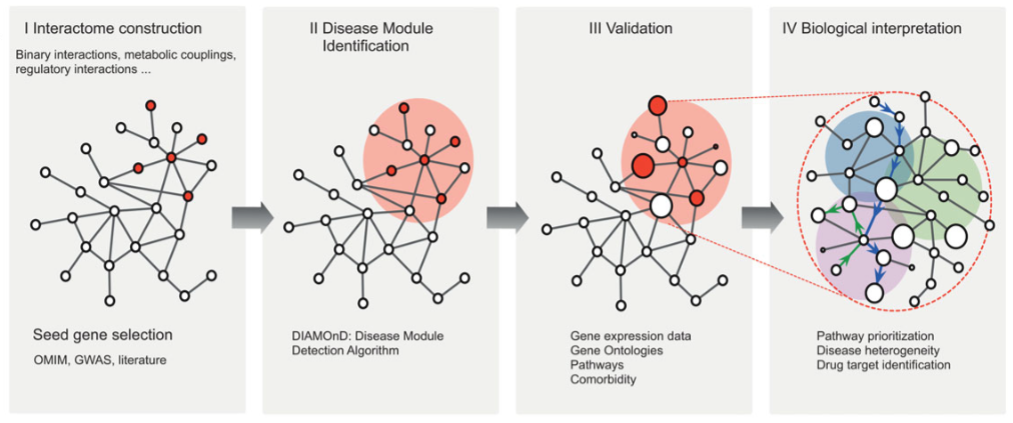
\includegraphics[width=0.5\linewidth]{images/network_module.png}
        \caption{Example of identifying a network module in the Human interactome.}
        \label{fig:example of a network module}
    \end{figure}
    
\item \textbf{Drug--target list.} The drug--target table of Cheng et al.\ \cite{cheng2019combinations}, filled in from ChEMBL \cite{zdrazil2024chembl} or DGIdb \cite{freshour2021dgidb} for any candidate it lacks. Only targets present in the interactome are kept.
\item \textbf{AD disease module.} The same definition as the sister project: genes from the largest recent AD genetic study \cite{bellenguez2022new} plus well-known AD genes (e.g., \textit{APP}, \textit{PSEN1}, \textit{PSEN2}, \textit{APOE}, \textit{MAPT}).
\item \textbf{Candidate list} (Decision D1). Either the sister project's ranked output, or a hand-picked (``curated'') list: repurposed drugs from the 2025 and 2026 AD pipeline reviews \cite{cummings2025pipeline,cummings2026pipeline}, the four approved symptomatic AD drugs (donepezil, rivastigmine, galantamine, memantine), and drugs suggested by published AD network studies \cite{fang2021sildenafil,csbj2023stages,lqt2025ad}. Antibody drugs whose targets are not in the interactome are left out.
\item \textbf{Scaling pool.} For speed experiments only: every drug in the drug--target table with at least one target in the interactome (expected: roughly a thousand).
\item \textbf{Settings.} Combination size $k\in\{2,3,4\}$ for biological results (up to 8 for speed tests); overlap weight $\lambda$; number of SA chains and steps; random seeds.
\end{itemize}


The solvers never see biology. They see a list of $n$ numbers (how close each drug is to AD), an $n\times n$ table (how much each pair of drugs overlaps), and the number $k$. Everything biological is a label attached to those numbers, with a note saying where it came from.



The pipeline answers one question: \emph{which $k$ drugs together cover the AD module best without overlapping each other?}

\begin{enumerate}
\item \textbf{Score each drug.} Take drug $i$'s closeness score $z_i$ (\Cref{app:formulation}). Only drugs with $z_i<0$ (closer than chance) are kept. The reward is $w_i=-z_i$, capped and scaled to the range 0--1.
\item \textbf{Score each pair.} Compute the separation $s_{ij}$ between the targets of drugs $i$ and $j$ \cite{menche2015uncovering}. Overlapping pairs ($s_{ij}<0$) get a penalty $P_{ij}=-s_{ij}$, scaled to 0--1; all other pairs get 0.
\item \textbf{Find the best team.} Find the set $\Sel$ of exactly $k$ drugs with the lowest energy
\begin{equation}
E(\Sel) = -\sum_{i\in\Sel} w_i + \lambda\sum_{\{i,j\}\subseteq\Sel} P_{ij}.
\label{eq:objective}
\end{equation}
The first sum rewards closeness to AD; the second punishes overlap. Low energy therefore means complementary exposure \cite{cheng2019combinations}.
\end{enumerate}


For three drugs A, B, C the energy is: minus (reward of A + reward of B + reward of C), plus $\lambda$ times (overlap of A--B + overlap of A--C + overlap of B--C). Pick the three drugs that make this number as small as possible.


\paragraph{(i) Processes parallelized with SIMD (AVX2) and SIMT (CUDA).}

\begin{enumerate}
\item \textbf{Exact search over all combinations} (Module 3, CUDA). The $\binom{n}{k}$ combinations are numbered in order and split into equal slices, one per GPU thread. Each thread finds its first combination from its slice number, walks through its slice, and remembers its best. The threads then combine their bests with a minimum reduction. A sequential C++ version gives the cross-check and the timing baseline.
\item \textbf{Simulated annealing} (Module 4, AVX2 and CUDA). Each chain holds exactly $k$ drugs and repeatedly tries swapping one chosen drug for one unchosen drug. A helper array $g$ of length $n$ makes the score change of any swap an $O(1)$ calculation (\Cref{app:classical}). When a swap is accepted, $g$ is updated with $g \leftarrow g + \lambda(P_{:,j}-P_{:,i})$, an array add and subtract over $n$ elements.
\begin{itemize}
\item \textbf{AVX2}: this update is a hand-written assembly loop using \texttt{ymm} registers, eight 32-bit integers per instruction.
\item \textbf{CUDA}: thousands of chains run at once. Version 1 uses one thread per chain.
\end{itemize}
\item \textbf{QAOA simulation} (Module 5). The cuStateVec library applies each quantum gate to all $2^n$ numbers of the simulated state in parallel on the GPU. We do not write this kernel, but we time it and measure its memory use.
\end{enumerate}

\paragraph{(ii) Related works and how this implementation differs.} Complementary exposure \cite{cheng2019combinations} and its quantum-annealing QUBO \cite{ramos2025quantum} give us the scoring idea. Optimized simulated annealing \cite{isakov2015optimised} and QAOA \cite{farhi2014qaoa} give us the solvers. Our implementation differs in that it:
\begin{itemize}
\item targets AD, and proves and tests that the QUBO gives the right answer instead of tuning its settings by trial and error;
\item searches only valid combinations in the classical solvers, so no penalty setting is needed there;
\item writes \emph{one} SA algorithm for scalar, SIMD and GPU hardware with shared random numbers and integer arithmetic, so the three versions make identical decisions and their run times can be compared fairly;
\item measures QAOA against the exact best answer on every instance, instead of reporting quantum results alone.
\end{itemize}

\paragraph{(iii) Parallelization plan.}

\begin{table}[ht]
\centering
\small
\begin{tabularx}{\linewidth}{>{\raggedright\arraybackslash}p{2.9cm}X>{\raggedright\arraybackslash}p{2.3cm}}
\toprule
Step & How the work is split & Limited by \\
\midrule
Exact search (GPU) & Combinations numbered $0,\dots,\binom{n}{k}-1$ and split into equal slices, one per thread. Each thread decodes its first combination, steps to the next one in order, and re-scores only the drugs that changed. Warp and block minimum reduction of (energy, combination number, tie count). & Arithmetic \\
SA, AVX2 & Per chain: drawing the random swap and computing its score change is scalar code. Accepted swaps update $g$ with \texttt{vmovdqa}/\texttt{vpaddd}/\texttt{vpsubd} over eight lanes, unrolled four times. & Share of steps accepted; memory bandwidth for large $n$ \\
SA, CUDA & One thread per chain; $g$ in the thread's local memory. & Uncoalesced memory access \\
QAOA & cuStateVec over $2^n$ numbers; the angle-tuning loop runs on the CPU. & GPU memory \\
\bottomrule
\end{tabularx}
\caption{Parallelization plan. Pseudocode and memory layouts are in \Cref{app:classical}.}
\label{tab:parplan}
\end{table}

Data moves to the GPU once (a few MB at most) and results come back once.

\paragraph{(iv) Processes not parallelized.}
\begin{itemize}
\item Downloading data, matching gene and drug identifiers, building the interactome and target lists.
\item Computing closeness scores for the curated list when the sister project's output is not used (a small Python script; not part of the contribution).
\item Shortest-path distances among target proteins and the separation table $s_{ij}$ (breadth-first search from a few thousand proteins at most; fast enough on the CPU).
\item Building the QUBO and Ising files and the annealing temperature schedule.
\item Building QAOA circuits and running the angle-tuning optimizer (COBYLA), which calls the GPU simulator.
\item Result analysis and plotting.
\end{itemize}

\subsubsection{Outputs}

\begin{enumerate}
\item \textbf{Problem files}: candidate table, separation and penalty tables, QUBO and Ising files, each with a record of where its numbers came from.
\item \textbf{Best AD combinations} for each $k$ and $\lambda$, with the exact best answer, how many combinations tie for best, and the runners-up.
\item \textbf{Execution-time comparison}: sequential C++ vs.\ AVX2 vs.\ CUDA for SA, and CPU vs.\ GPU for exact search, across $n$ and $k$, with speedup charts.
\item \textbf{Correctness report}: CPU and GPU exact search agree; all SA versions make identical decisions; QUBO and Ising scores agree for every yes/no pattern on small problems.
\item \textbf{QAOA results}: how often QAOA finds the best combination, the share of valid answers, and simulator time and memory, for each depth $p$ and size $n$.
\end{enumerate}
